% Example of the BIO labelling (Figure 3 of the paper)
\begin{figure}[t]
\centering
\resizebox{\columnwidth}{!}{%
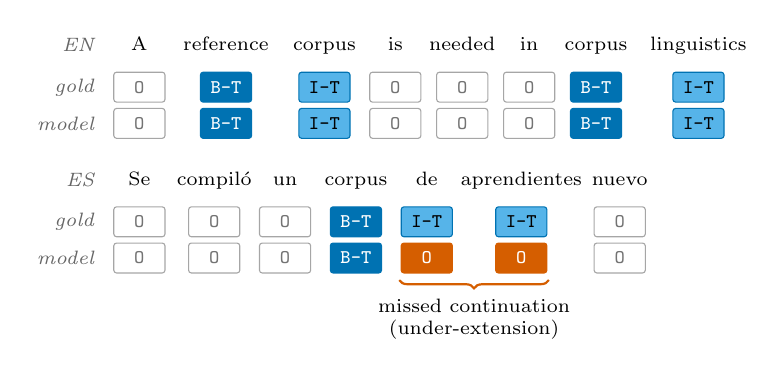
\begin{tikzpicture}[
  font=\rmfamily\scriptsize,
  tok/.style={inner sep=1.5pt, minimum height=4.2mm, anchor=base},
  et/.style={draw=black!35, rounded corners=1pt, inner sep=1.4pt, minimum width=6.5mm,
             minimum height=3.8mm, font=\ttfamily\scriptsize},
  O/.style={et, fill=white, text=black!55},
  B/.style={et, fill={rgb,255:red,0;green,114;blue,178}, draw={rgb,255:red,0;green,114;blue,178}, text=white, font=\ttfamily\scriptsize\bfseries},
  I/.style={et, fill={rgb,255:red,86;green,180;blue,233}, draw={rgb,255:red,0;green,114;blue,178}, text=black, font=\ttfamily\scriptsize\bfseries},
  fila/.style={font=\rmfamily\scriptsize\itshape, text=black!60, anchor=east},
  err/.style={et, fill={rgb,255:red,213;green,94;blue,0}, draw={rgb,255:red,213;green,94;blue,0}, text=white, font=\ttfamily\scriptsize\bfseries}
]
% ── English example ──
\foreach \x/\w/\t/\l in {0.5/A/O/O, 1.6/reference/B/B-T, 2.85/corpus/I/I-T, 3.75/is/O/O, 4.6/needed/O/O, 5.45/in/O/O, 6.3/corpus/B/B-T, 7.6/linguistics/I/I-T} {
  \node[tok] at (\x, 0) {\w};
  \node[\t] at (\x, -0.46) {\l};
  \node[\t] at (\x, -0.92) {\l};
}
\node[fila] at (0.05, 0.07) {EN};
\node[fila] at (0.05, -0.46) {gold};
\node[fila] at (0.05, -0.92) {model};

% ── Spanish example, with a wrong prediction ──
\foreach \x/\w/\t/\l/\tp/\lp in {0.5/Se/O/O/O/O, 1.45/compiló/O/O/O/O, 2.35/un/O/O/O/O, 3.25/corpus/B/B-T/B/B-T, 4.15/de/I/I-T/err/O, 5.35/aprendientes/I/I-T/err/O, 6.6/nuevo/O/O/O/O} {
  \node[tok] at (\x, -1.71) {\w};
  \node[\t] at (\x, -2.17) {\l};
  \node[\tp] at (\x, -2.63) {\lp};
}
\node[fila] at (0.05, -1.64) {ES};
\node[fila] at (0.05, -2.17) {gold};
\node[fila] at (0.05, -2.63) {model};
\draw[decorate, decoration={brace, amplitude=3pt, mirror}, draw={rgb,255:red,213;green,94;blue,0}, thick]
  (3.8, -2.91) -- (5.7, -2.91) node[midway, below=3pt, font=\rmfamily\scriptsize, text=black, align=center]
  {missed continuation\\(under-extension)};
\end{tikzpicture}}
\caption{The \texttt{BIO} scheme: \texttt{B-T} marks the first word of a term, \texttt{I-T} the words that continue it and \texttt{O} the rest. In the English example, the model recognises both terms; in the Spanish one, it labels only the known nucleus of the reserved term \textit{corpus de aprendientes}, the most frequent partial error on unseen terms.}
\label{fig:bio}
\end{figure}
